\chapter{Neurónové siete}


Neurónová sieť je založená na orientovanom grafe (ako je možné vidieť na obrázku \ref{fig:nn}), je teda zložená z uzlov, ktoré sú spojené orientovanými hranami \citep{rnn:spol}.
Spojenie uzlu $i$ do uzlu $j$ slúži na propagáciu aktivácie $a_i$ z $i$ do $j$.
Každé takéto spojenie má priradenú váhu $w_{i,j}$, ktorá rozhoduje o sile a znamienku spojenia.
Každý uzol má naviac falošný vstup $a_0=1$ s priradenou váhou $w_{0,j}$.
Všetky uzly si potom vypočítajú váženú hodnotu vstupov, pre uzol $j$ je táto hodnota:
$$in_j=\sum^n_{i=0}w_{i,j}a_i$$
Potom sa na výsledok aplikuje aktivačná funkcia g, tým získame výstup z uzlu:
$$a_j=g(in_j)=g\left(\sum^n_{i=0}w_{i,j}a_i\right)$$

\begin{figure} [h!]
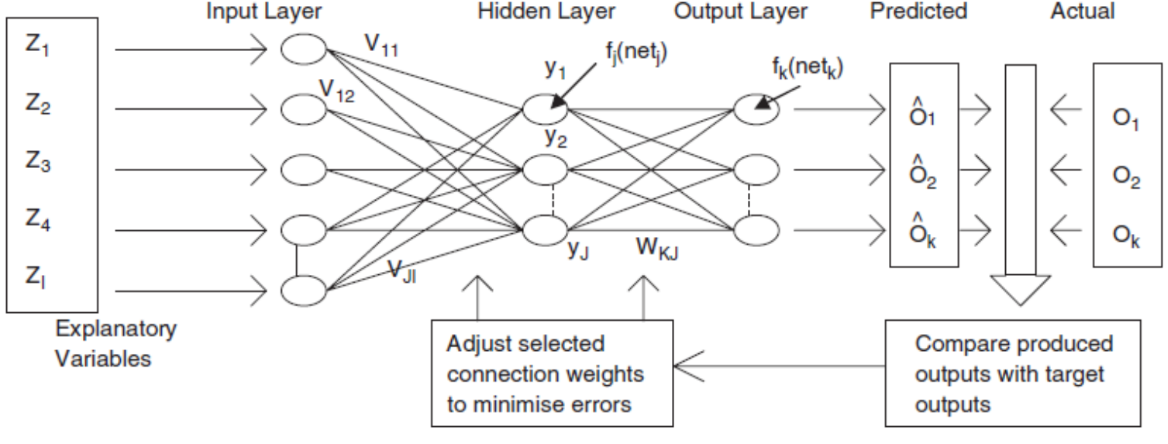
\includegraphics[width=\textwidth]{../img/nn.png}
\caption{Ukážka jednej z neurónových sietí}
\label{fig:nn}
\end{figure}

Aktivačná funkcia $g$ je typicky buď pevná hranica alebo logistická funkcia.
V prvom prípade sa uzly volajú perceptrony, v druhom prípade sa niekedy používa pojem \textit{sigmoid perceptron}.
Obe tieto typy nelineárnych aktivačných funkcií zaručujú dôležitú vlastnosť neurónovej siete, a to, že celá sieť uzlov môže reprezentovať aj nelineárnu funkciu.

\begin{figure} [h!]
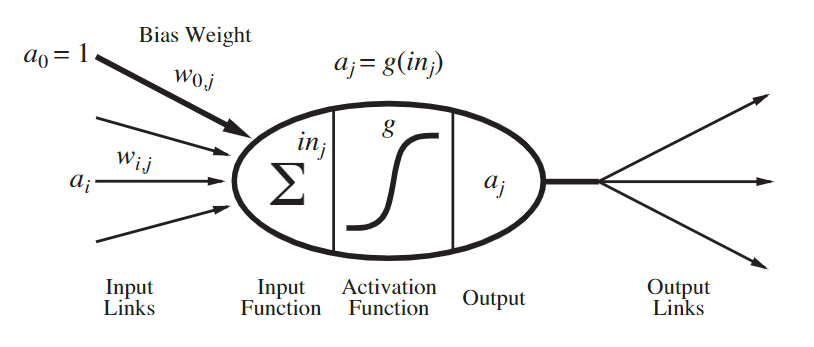
\includegraphics[width=\textwidth]{../img/nn_aima_neuron.png}
\caption{Takto vyzerá jeden uzol siete (neurón) \citep{aima}.}
\end{figure}

Takto teda vyzerá matematický model jedného uzlu (v tomto prípade zvaného neurón) v sieti.
Spájanie týchto neurónov vytvorí sieť.
Existujú rôzne spôsoby, akými sa dajú jednotlivé neuróny spojiť do siete.
Dva z nich sú dôležité pre túto prácu, pretože obe použijeme a porovnáme medzi sebou.
Tieto dva prístupy sú dopredná a rekuretná neurónová sieť.

\section{Dopredné neurónové siete}
Dopredná neurónová sieť (feed-forward neural network ) má spojenia len v jednom smere, takže tvorí orientovaný acyklický graf (obrázok \ref{fig:nn} zobrazuje práve tento typ siete).
Ak si graf topologicky usporiadame, tak každý uzol dostane vstup z niektorých z predchádzajúcich uzlov a predá výstup niektorým z nasledujúcich uzlov.
Dopredná neurónová sieť teda predstavuje funkciu jej momentálneho vstupu, teda neuchováva žiaden stav, ak nepočítame váhy samotné \citep{aima}.

Tieto siete sú obvykle zoradené do vstiev tak, že každý neurón dostane vstup len z neurónov z predošlej vrstvy.
Podľa počtu vrstiev sa siete delia na jednovrstvové a viacvrstvové .

\subsection{Jednovrstvové siete}
Jednovrstvové siete spájajú vstupné neuróny priamo s výstupnými.
Tieto siete sú ale obmedzené a nevedia sa naučiť funkcie, ktoré nie sú lineárne separabilné, platí to dokonca aj pre niektoré jednoduché funkcie ako napríklad XOR \citep{aima}. 

V Euklidovskej geometrii je lineárna separabilita vlastnosť dvoch množín bodov v priestore, ktoré sa dajú presne oddeliť nadrovinou v tomto priestore. 
Najjednoduchšie sa to dá predstaviť v dvojrozmernom priestore napríklad na boolovskej funkcii OR. Bodu (0,0) v súradnicovom systéme (x,y) priradí funkcia hodnotu 0, bodom (1,0), (0,1) a (1,1) priradí hodnotu 1. Ak body rozdelíme do množín podľa priradenej hodnoty, tak tieto dva množiny sa dajú presne oddeliť priamkou, napríklad $y = -x + 1/2$. Je zjavné, že množiny bodov získané z funkcie XOR (tabuľka \ref{xor}) sa takto rozdeliť nedajú, tieto množiny teda nie sú lineárne separabilné.

\begin{table}[h]
\begin{center}
\begin{tabular}{ |c|c|c| } 
 \hline 
 x & y & x XOR y \\ 
 \hline
 0 & 0 & 0 \\ 
 0 & 1 & 1 \\ 
 1 & 0 & 1 \\ 
 1 & 1 & 0 \\ 
 \hline
\end{tabular}
\caption{Tabuľka funkcie XOR}
\label{xor}
\end{center}
\end{table}

\subsection{Viacvrstvové siete}
Viacvrstvové siete majú medzi vstupom do siete a výstupom z nej ešte jednu alebo viac vrstiev tzv. skrytých (hidden) neurónov (Obrázok \ref{img:single}).
Waren McCulloch a Walter Pitts \citep{multi} vo svojom článku dokázali, že jeden neurón v sieti vie reprezentovať základné boolovské funkcie AND, OR a NOT a vyslovili, že každá dodatočná funkcionalita sa dá získať spojením väčšieho počtu neurónov do siete. Samotné XOR z predchádzajúcej podsekcie sa dá vyjadriť ako 
\textit{(x OR y) AND (NOT(x) OR NOT(y))} a podľa tohto vieme vytvoriť aj jednoduchú viacvrstvovú sieť, ktorá používa len neuróny s týmito funkciami (obrázok \ref{img:xor}, matematika týchto viacvrstvových modelov nám však dovoľuje vytvoriť aj jednoduchšie siete pre rozoznávanie XOR, je len potrebné zmeniť aktivačnú funkciu a váhy jednotlivých spojení).

\begin{figure}  [h!]
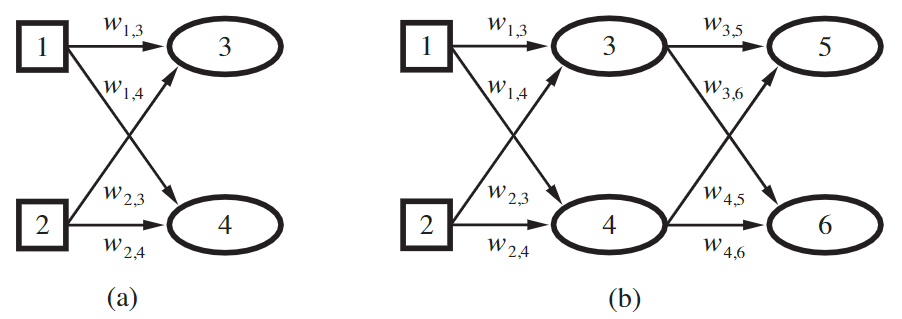
\includegraphics[width=\textwidth]{../img/nn_aima_single_multi.png}
\caption{Ukážka rozdielu medzi jednovrstvou(a) a viacvrstvovou sieťou (b). Obe majú 2 vstupné a 2 výstupné neuróny, viacvrstvová má ešte medzi nimi ďalšie vrstvy skrytých neurónov (v tomto prípade jednu vrstvu s 2 skrytými neurónmi), falošné vstupy do každého neuŕony nie sú ukázané \citep{aima}.}
\label{img:single}
\end{figure}

\begin{figure}  [h!]
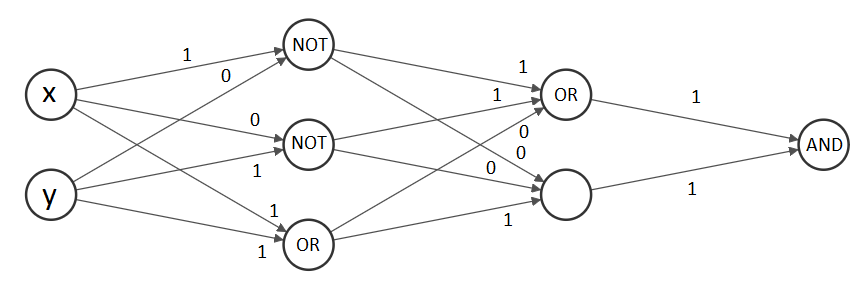
\includegraphics[width=\textwidth]{../img/xor.png}
\caption{Jednoduchá ukážka viacvrstvovej neurónovej siete rozoznávajúcej XOR.}
\label{img:xor}
\end{figure}


\section{Rekurentné neurónové siete}
Na druhej strane máme rekurentnú neurónovú sieť (\textit{RNN}).
Tento typ siete posúva svoj výstup naspäť do svojho vlastného vstupu (obrázok \ref{rnn}). 
Z toho vyplýva, že aktivačné úrovne siete tvoria dynamický systém, ktorý môže dosiahnuť stabilný stav alebo oscilovať či sa dokonca správať chaoticky.
\begin{figure} 
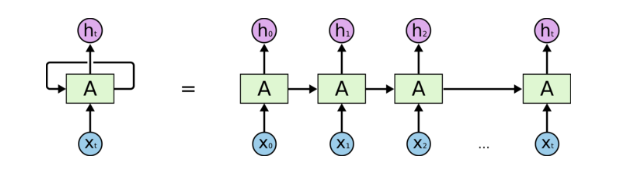
\includegraphics[width=\textwidth]{../img/rnn.png}
\caption{Jednoduchá ukážka rekurentnej neurónovej siete. $A$ je sieť, $x_i$ je jej vstup a $h_i$ je jej výstup. Sieť si predáva medzi výpočtom výstupov stav (vodorovné šípky) \citep{rnn:colah}.}
\label{rnn}
\end{figure}

Výstup siete závisí na vstupe. 
Pri tomto type siete môže výstup závisieť aj na predchádzajúcich výstupoch, tranzitívne teda aj na predchádzajúcich vstupoch.
Z toho vyplýva, že si rekurentná neurónová sieť môže vypracovať krátkodobú pamäť \citep{aima}.

RNN sa používa tam, kde dopredná neurónová sieť zlyháva, a to keď nám záleží na závislosti na predchádzajúcich vstupoch. 
Príklady použitia sú napríklad predikcia nasledujúceho slova v texte, rozpoznávanie reči alebo preklad textu medzi jazykmi.
Ako príklad si môžeme predstaviť slovné spojenie \uv{mraky sú na nebi}. 
Ak by sme predpovedali posledné slovo z tohto slovného spojenia, tak by nám nestačilo poznať len posledné slovo, ale aj pár predchádzajúcich. 
Tento prípad ukazuje krátkodobé závislosti jednotlivých slov, teda slová, ktoré na sebe závisia sú v krátkej vzdialenosti od seba (na obrázku \ref{rnn:std} môžeme vidieť príklad RNN na vyhodnocovanie krátkodobých závislostí).
\begin{figure}  [h!]
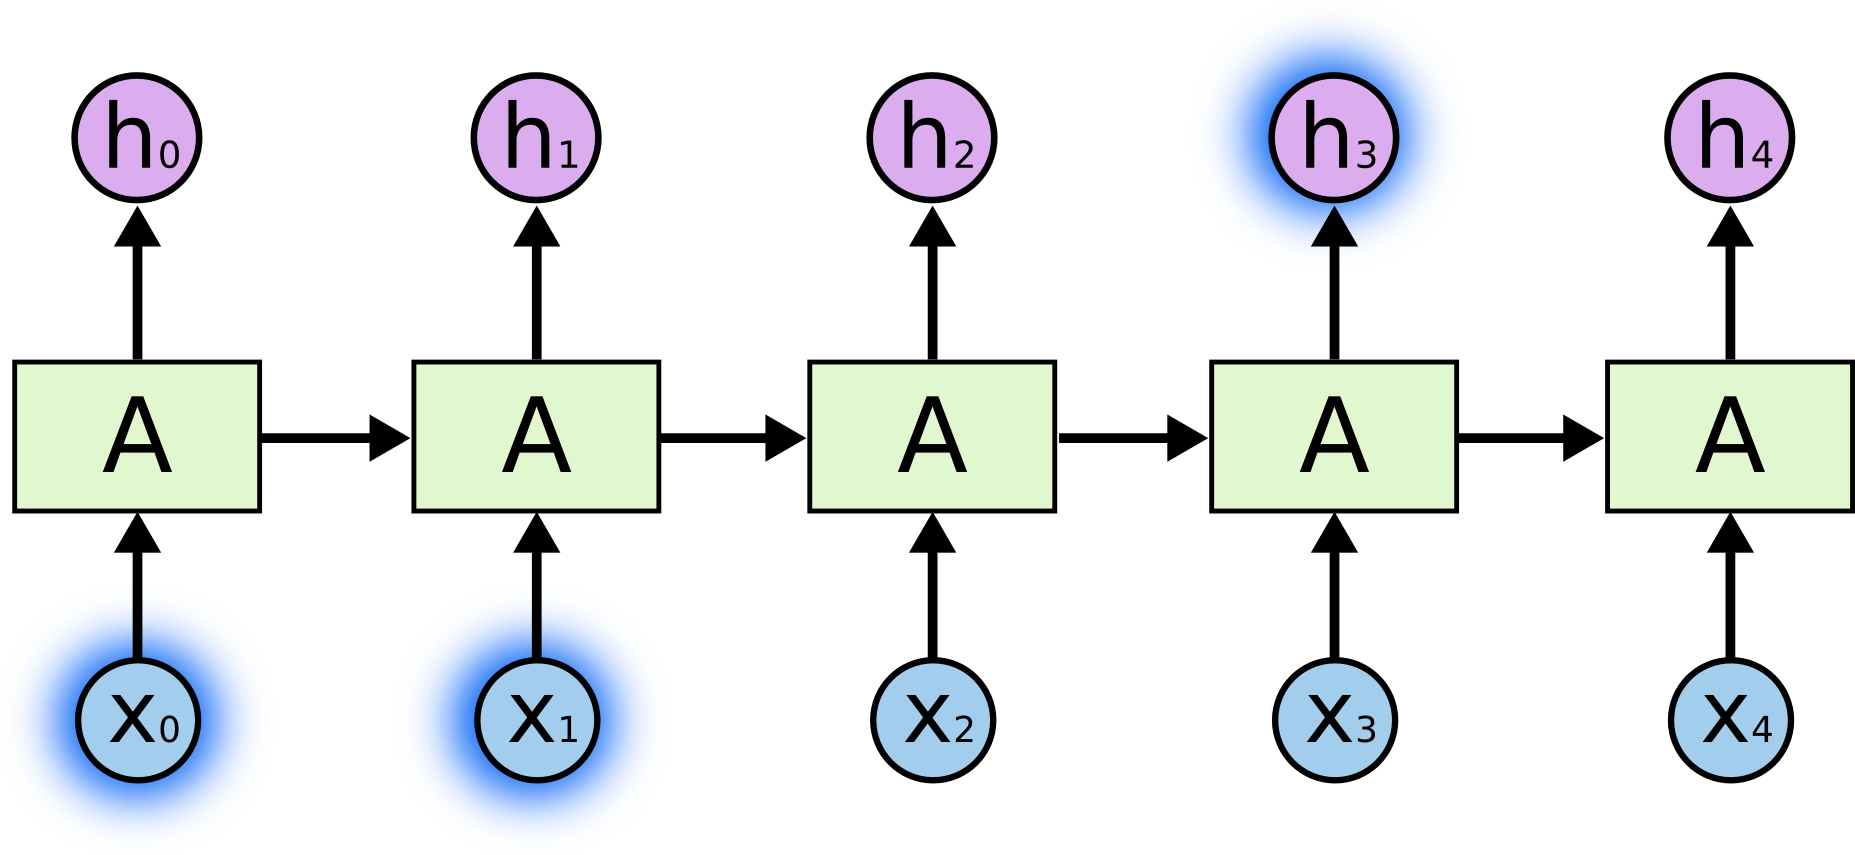
\includegraphics[width=\textwidth]{../img/rnn-std.png}
\caption{Ukážka krátkodobej závislosti, výstup $h_3$ závisí na vstupoch $x_0$ a $x_1$ \citep{rnn:colah}.}
\label{rnn:std}
\end{figure}

Pri doprednej neurónovej sieti by sme to vedeli dosiahnuť, ale potrebovali by sme zafixovať počet slovných n-gramov, ktoré by sme použili a každý ďalší by zvýšil výpočetnú náročnosť. Ak by sme mali napríklad slovné spojenie \uv{mraky sú na modrom nebi}, tak na predikciu posledného slova by sme si museli uchovávať informáciu o posledných 4 slovách, čo je o jedno viac ako pri poslednom príklade.

V prípade RNN nám stačí vždy vyhodnocovať posledné slovo a predávať si nejaký stav, ktorý sieť má. Pre náš príklad by sme si mohli posúvať informáciu o tom, že hovoríme o mraku. Všeobecne pri predikcii nasledujúceho slova v texte by sme si ideálne chceli uchovávať informáciu o gramatických kategóriách dôležitých slov, pretože v slovenčine aj češtine je táto informácia dôležitá pre vytvorenie správneho tvaru predikovaného slova, nakoľko sa gramatické kategórie medzi vetnými členmi, ktoré sú spolu v syntaktickom vzťahu, musia zhodovať.

Teoreticky sme schopní vytvoriť RNN, ktorá si pamätá závislosť na jednotlivých slovách s ľubovoľnou vzdialenosťou medzi jednotlivými slovami (ľubovoľným počtom slov medzi nimi). Nanešťastie v praxi to nefunguje až tak ideálne, vo svojej práci to ukázali Bengio, Simard a Frasconi už v roku 1994 \citep{rnn:bengio}.
Pre príklad si môžeme predstaviť text, kde sa niekde na začiatku objaví veta \uv{Narodil som sa vo Francúzsku.}, potom nasleduje nejaký text a o pár viet ďalej nasleduje časť \uv{...hovorím plynule francúzsky}. Ak by sme sa pokúsili predpovedať posledné uvedené slovo, možno by sme sa dozvedeli, že chceme nejaký jazyk, ale v šume zo všetkých slov medzitým by sme stratili informáciu o krajine \citep{rnn:colah}.
Tento príklad predstavuje tzv. dlhodobé závislosti (na obrázku \ref{rnn:ltd} môžeme vidieť príklad dlhodobej závislosti v RNN).


\begin{figure}  [h!]
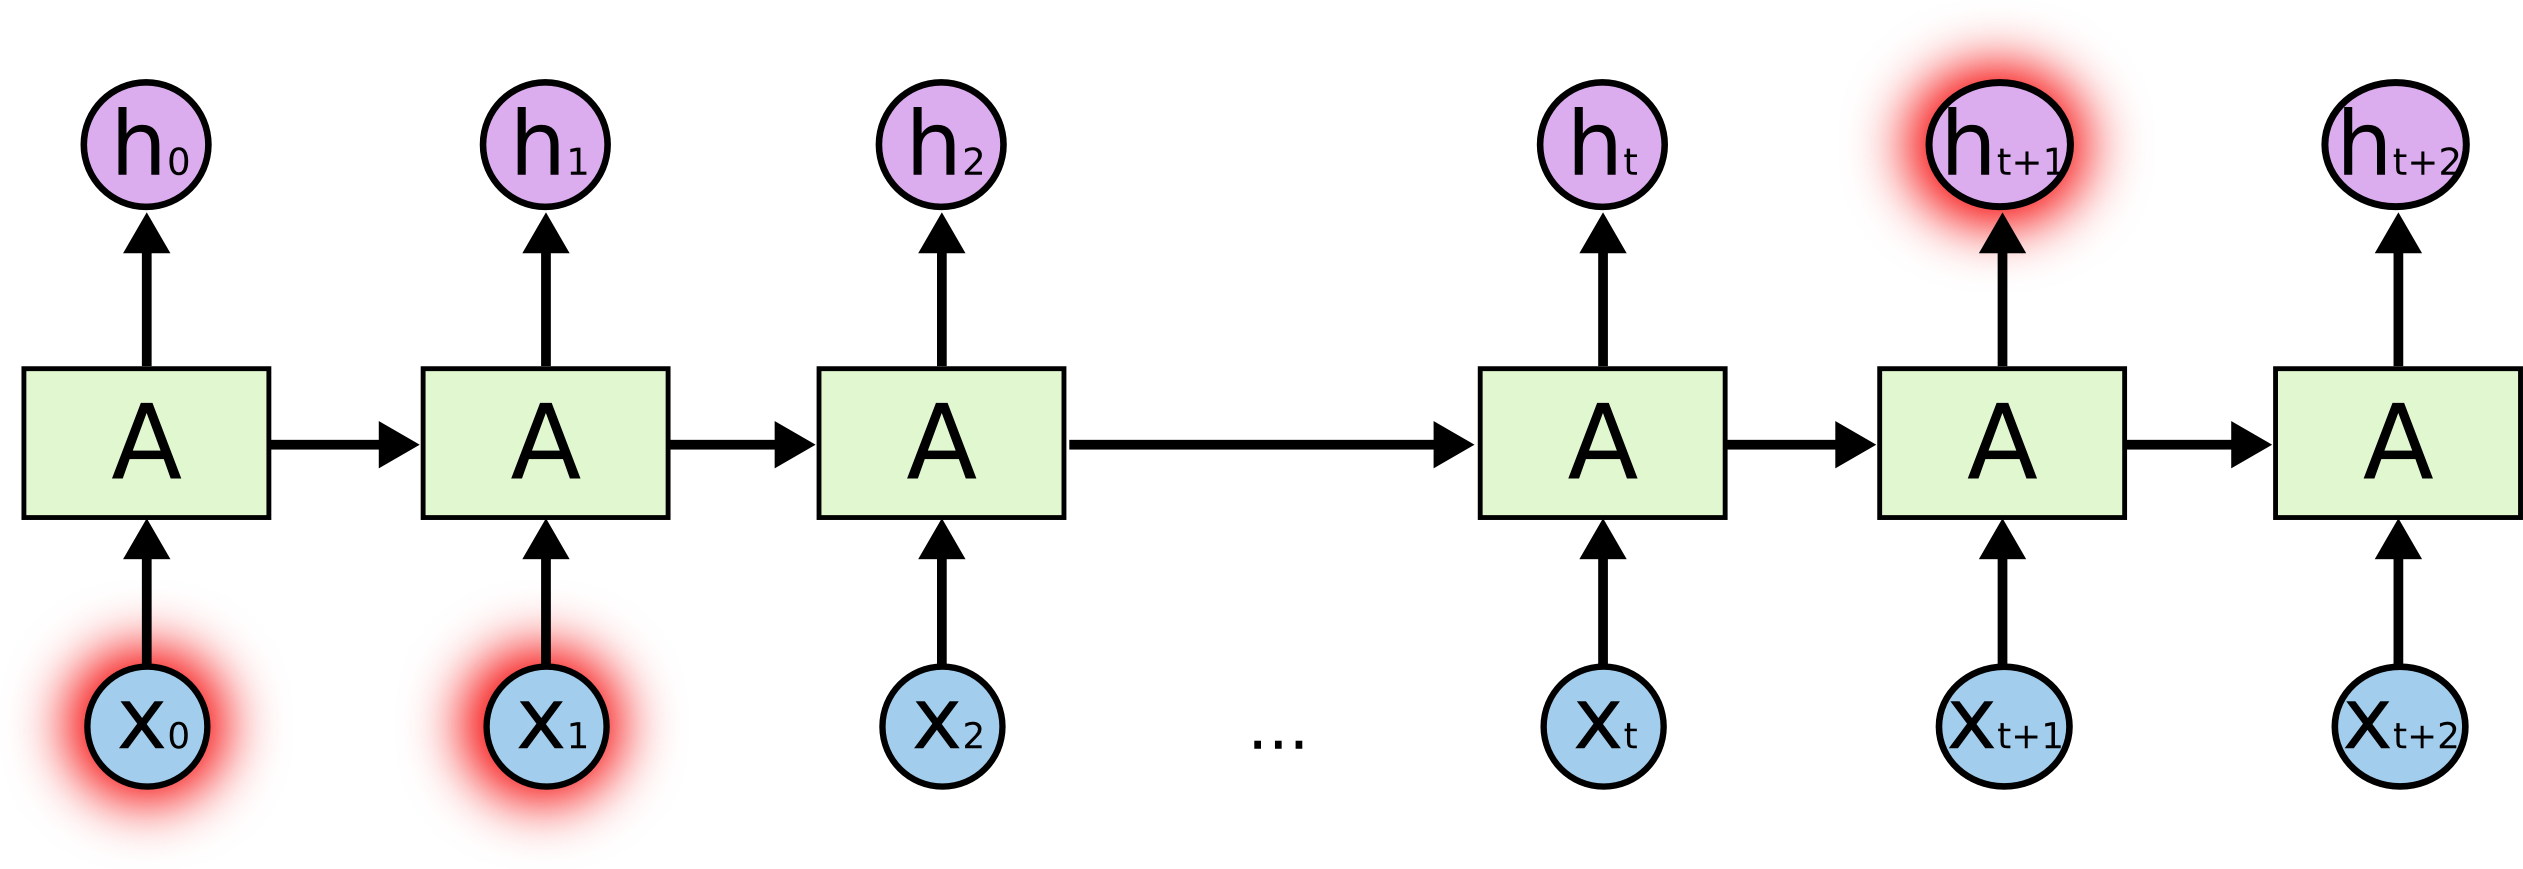
\includegraphics[width=\textwidth]{../img/rnn_ltd.png}
\caption{Ukážka dlhodobej závislosti, výstup $h_{t+1}$ závisí na vstupoch $x_0$ a $x_1$ \citep{rnn:colah}.}
\label{rnn:ltd}
\end{figure}

\subsection{LSTM}
LSTM (skratka pre \textit{Long Short-Term Memory} voľne preložiteľné ako ďaleká krátkodobá pamäť) je špeciálnym typom RNN skonštruovaným tak, aby mal čo najmenšie problémy pri dlhodobej závislosti \citep{rnn:colah}. 
Predstavili ich v roku 1997 vo svojej práci Hochreiter a Schmidhuber \citep{rnn:hoch}.
Všetky štandartné RNN majú veľmi jednoduchú reťazovú štruktúru, napríklad na vstup a stav siete (posledný výstup siete) aplikujú funkciu $tanh$ a výsledok pošlú na výstup a ako stav ďalšej sieti (príklad je vidieť na obrázku \ref{simple_rnn}). 
\begin{figure}  [h!]
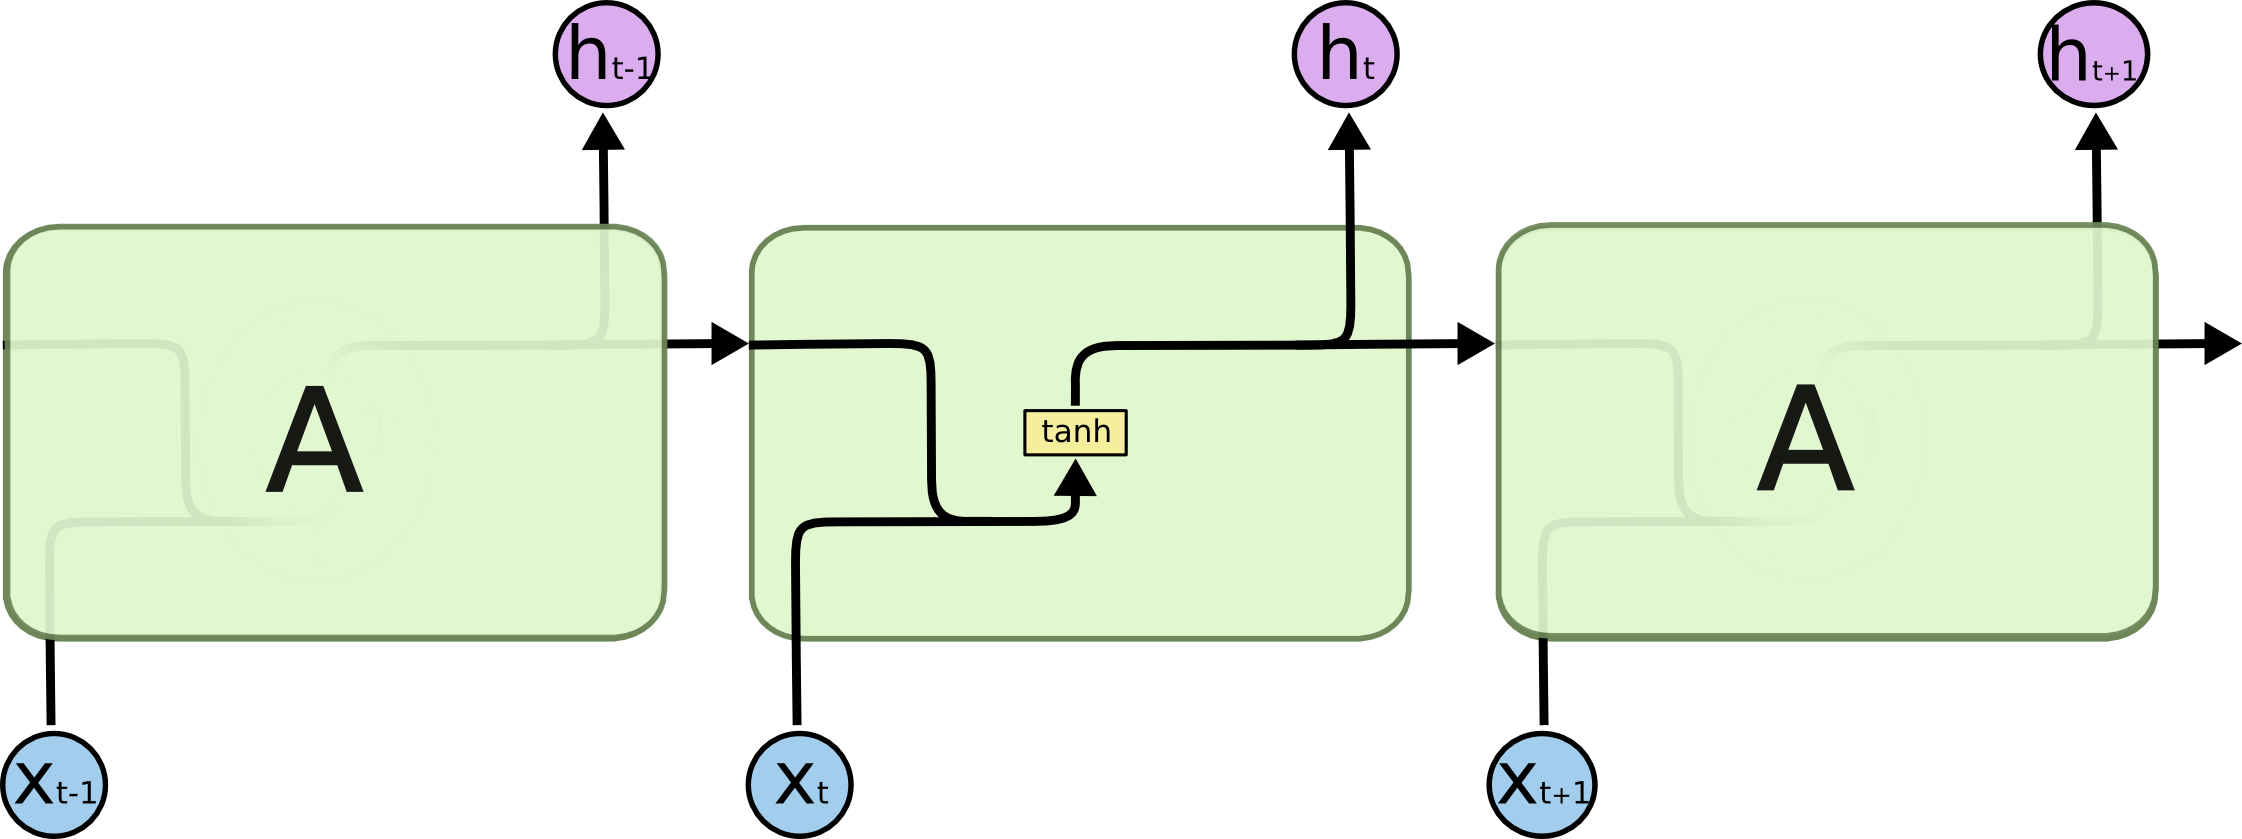
\includegraphics[width=\textwidth]{../img/simple_rnn.png}
\caption{Ukážka ako vyzerá jednoduchá RNN zvnútra \citep{rnn:colah}.}
\label{simple_rnn}
\end{figure}

LSTM má tiež reťazovú štruktúru, ale obvykle funguje mierne komplikovanejšie, namiesto jednej vrstvy, ktorá aplikuje nejakú funkciu na vstup a stav siete, obsahuje hneď 4 vrstvy (príklad jednej z možných prevedení LSTM je na obrázku \ref{lstm}).
\begin{figure}  [h!]
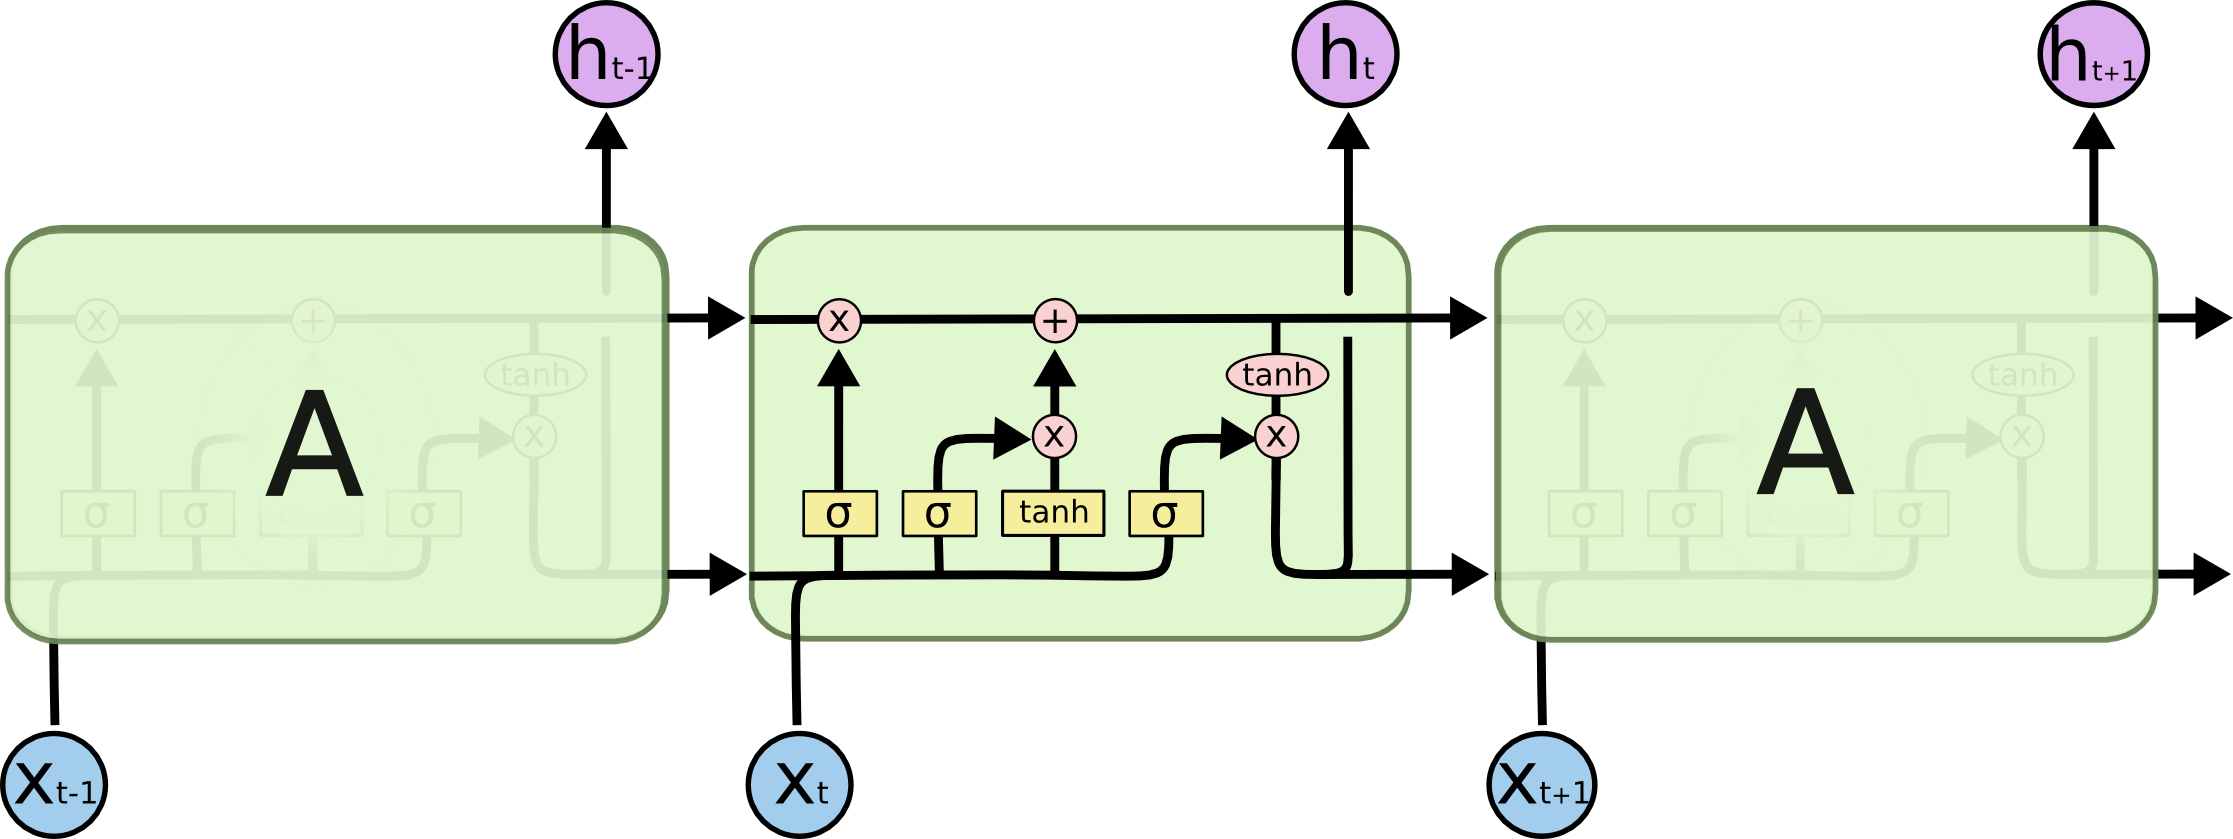
\includegraphics[width=\textwidth]{../img/lstm.png}
\caption{Ukážka jedného zo spôsobov implementácie LSTM zvnútra \citep{rnn:colah}.}
\label{lstm}
\end{figure}

\begin{figure} [h!]
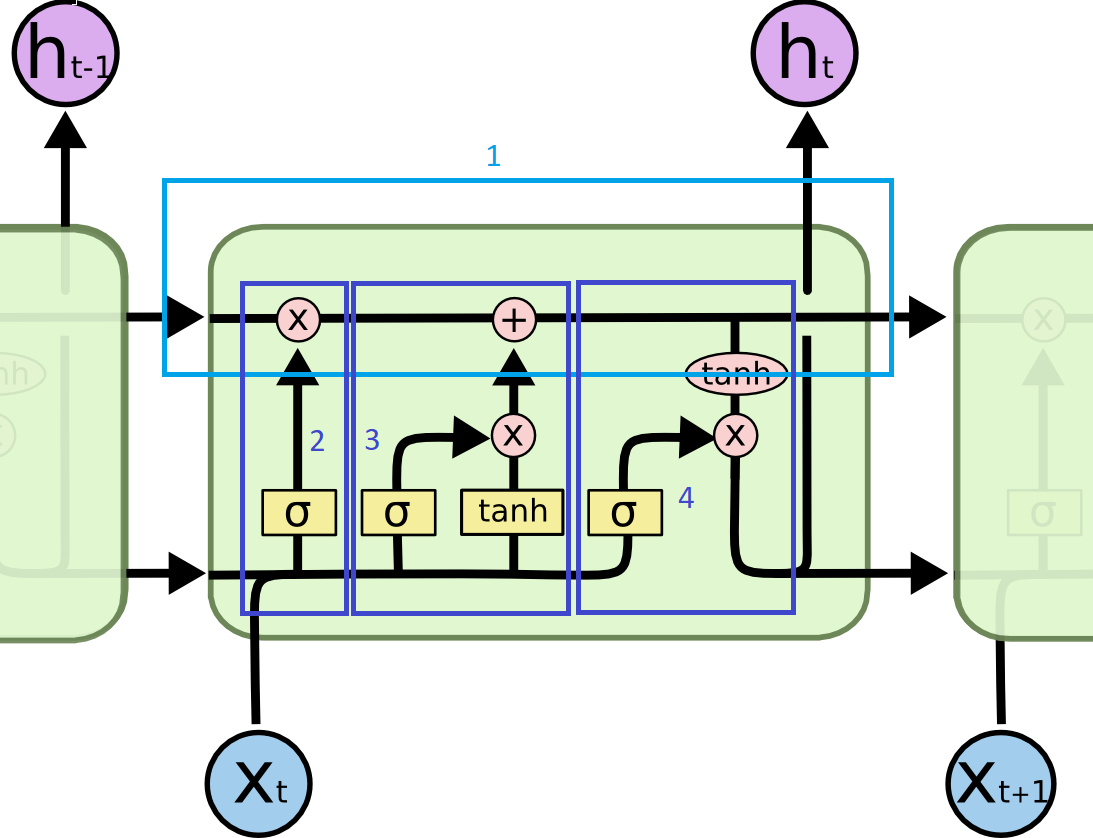
\includegraphics[width=\textwidth]{../img/lstm-close.png}
\caption{Ukážka prezentovaného spôsobou RNN rozdelená na 4 časti.}
\label{lstm:close}
\end{figure}

Základom LSTM je stav siete (na obrázku \ref{lstm:close} úsek označený číslom 1).
Tento stav pokračuje cez celú sieť až na koniec iba s miernými zmenami.
Veľmi jednoducho sa môže stať, že sa stav počas výpočtu skoro nezmení.


LSTM má schopnosť odstrániť stav alebo pridať do neho nejakú informáciu pomocou štruktúr zvaných brány. Brány predstavujú spôsob ako môže informácia prejsť. 
Sú zložené zo sigmoidovej $\sigma$ vrstvy a násobení po zložkách. Výstup $\sigma$ funkcie je $x \in (0,1)$, takže číslo blízko nuly znamená, že skoro žiadna informácia sa nedostane ďalej a číslo blízko jednotky znamená, že prejde skoro všetko (na obrázku \ref{lstm:close} môžeme vidieť 3 takéto brány).

Prvým krokom je rozhodnúť, ktoré informácie sa nedostanú ďalej zo stavu siete. Toto rozhodnutie robí tzv. zabúdacia brána (na obrázku \ref{lstm:close} označená číslom 2). Tá sa pozrie na vstup $x_t$ a posledný výstup $h_{t-1}$ a na základe týchto čísel sa rozhodne, nakoľko ponechá stav siete.

Keď si predstavíme model predikcie nasledujúceho slova, tak jedným zo stavov siete môže byť rod predmetu, o ktorom je momentálny text, to je potrebné, aby sme mohli použiť správne zámeno, ak sa budeme naň odkazovať. Ak na vstup príde predmet alebo nový podmet, je pravdepodobne na čase zabudnúť starú informáciu o rode a pridať novú \citep{rnn:colah}.

O pridanie novej informácie sa stará ďalšia vrstva v sieti (na obrázku označená číslom 3). Táto vrstva sa skladá z tzv. vstupnej brány, ktorá sa stará o to, ktoré informácie si ponecháme a $tanh$ vrstva, ktorá vytvára vektor nových kandidátov, ktoré by mohli byť pridané do stavu.

Stav siete teda upravíme nasledovne: najprv ho prenásobíme hodnotou $x_{f_t}$, ktorá je výstupom zabúdacej brány a potom pripočítame do stavu nové informácie. Tento stav sa potom posúva ako stav do ďalšej iterácie.

Nakoniec sa musíme rozhodnúť, čo pôjde na výstup siete. Najprv prejde stav cez funkciu $tanh$, ktorá stlačí hodnoty stavu medzi -1 a 1 a potom prejde poslednou bránou (na obrázku \ref{lstm:close} označenou číslom 4), tá rozhodne, ktorá časť stavu pôjde na výstup \citep{rnn:colah}.

V našom príklade sme teda dostali ďalší predmet. Na výstup by sieť podľa toho, aký vetný člen očakáva, že bude nasledovať, mohla predať relevatné informácie o gramatických kategóriách. Stav môže naďalej obsahovať všetky tieto informácie.


\section{Učenie} \label{learn}
V predchádzajúcich sekciách sme hovorili o nastavení váh jednotlivých spojení medzi neurónmi a výbere aktivačnej funkcie.
V praxi si ale tieto hodnoty obvykle nenastavujeme manuálne, ale nastavuje si ich sieť sama procesom zvaným učenie. Neurónová sieť je učená iteratívnym spôsobom. 
V každej iterácii dostane sieť množinu vstupov.
Pre každý vstup vypočíta hodnotu odhadovaného výstupu, potom sa sieť pozrie na očakávaný výstup a zapamätá si rozdiel týchto hondôt.
Po skončení iterácie sa sieť pozrie na hodnoty týchto rozdielov a upraví si svoje váhy tak, aby nabudúce pri rovnakých dátach vydala výstup bližší k očakávanému výstupu.
Proces by mal naučiť sieť ohodnotiť celý dátaset čo najpresnejšie.
Ak dáta dobre reprezentujú celý problém a nie len nejakú jeho časť, tak sa môže naučiť generalizovať, teda vydať správny výstup aj na dáta, ktoré predtým nikde nevidela.

Konkrétnejšie, proces učenia začne inicializáciou váh. Váhy sa obvykle inicializujú náhodne.
Po inicializácii začne už spomínaný iteratívny proces.
V každom kroku zvolíme príslušnú podmnožinu trénovacích dát (\textit{batch}) a vyhodnotíme vypočítané výstupy porovnaním s očakávanými a pozmeníme jednotlivé váhy podľa toho.
Vypočítané výstupy sa vyhodnocujú pomocou stratovej funkcie.
Našou úlohou je hodnoty stratovej funkcie minimalizovať.
Jednou z najpoužívanejších stratových funkcií je stredná štvorcová chyba (\textit{Mean Squared Error}). Táto funkcia je definovaná ako funkcia $$MSE(x,y,f) = \frac{1}{m} \cdot \sum_{i=1}^m (f(x)_i - y_i)^2$$
kde
$f: \mathbb{R}^n \to \mathbb{R}^m$ je funkcia, ktorú simuluje neurónová sieť, $x \in \mathbb{R}^n$ vstupný vektor a $y \in \mathbb{R}^m$ očakávaná hodnota výstupu.
To je hodnota MSE pre jeden vstup, ale my trénujeme v podmnožinách vstupných dát veľkosti $k$ a až potom vyhodnocujeme. 
Pre tento prístup je MSE definovaná $$MSE(X,Y,f) = \frac{1}{k} \cdot \sum_{j=1}^k (MSE(X_j,Y_j,f)) = \frac{1}{k} \cdot \sum_{j=1}^k (\frac{1}{m} \cdot \sum_{i=1}^m  (f(X_j)_i - Y_{j_i})^2)) $$
kde $X \in \mathbb{R}^k \times \mathbb{R}^n$ je množina vstupných vektorov a $Y \in \mathbb{R}^k \times \mathbb{R}^m$ je množina očakávaných výstupov.

Na riešenie klasifikačných problémov, teda problémov, kde výstupom je vektor, ktorý obsahuje samé 0 a jednu 1, ktorá určuje, do ktorej triedy je vstup zaradený (ako v našom prípade, kde klasifikujeme zápasy na výhry, prehry a v prípade futbalu aj remízy), sa používa softmaxová strata.
Softmaxová strata (niekde v literatúre aj \textit{cross-entropy loss}) sa aplikuje len, keď je aktivačná funkcia vo výstupných neurónoch softmax $\sigma$. 
Softmax $\sigma: \mathbb{R}^k \to \mathbb{R}^k$ je daná ako $$\sigma(z)_i = \frac{e^{z_i}}{\sum_{j=1}^k e^{z_j}}$$
Vlastnosti tejto funkcie ukazujú, že súčet všetkých zložiek výstupného vektoru je 1, takže táto funkcia v prípade neurónových sietí ukazuje názor siete na to, ako pravdepodobné je, že sa vstup nachádza v triede $i$ $\forall i \in {1,\dots , k}$.
Na konci sa vždy upraví výstup softmaxu tak, aby bol výsledný vektor vhodný výstupu (teda najvyššia hodnota sa premení na 1, zvyšné na 0). Označme si tento výstupný vektor ako $v$.
Keď je súčet zložiek rovný 1, vieme použiť funkciu na výpočet entropie ($ H = -\sum_{i=1}^k \left(x_i \cdot log_2(x_i)\right) $).
Takže softmaxová stratová funkcia vyzerá nasledovne ($p \in {1,\dots, k}$ je $argmax_{\sigma(z)}$)
$$L(x,y) = -\sum_{i=1}^k \left(v_i*log_2(\sigma(z)_i)\right) = -\sum_{i=1}^k log_2\left(\frac{e^{z_p}}{\sum_{j=1}^k e^{z_{j}}}\right)  $$

Ďalšie masívne používané stratové funkcie sú 
absolútna strata ($L(x,y,f) = $ $\frac{1}{m}\sum_{i=1}^m \left|f(x)_i - y_i\right|$), 
$\epsilon$-necitlivá strata ($L(x,y,f) = \frac{1}{m}\sum_{i=1}^m \left(\left|f(x)_i - y_i\right| - \epsilon\right)$), 
logistická strata ($L(x,y,f) = \frac{1}{m} \sum_{i=1}^m  \left((ln(2))^{-1}\cdot ln(1+e^{-f(x)_iy_i})\right) $)
\citep{loss}.

Jedným zo spôsobov, ktoré sa používajú na úpravu jednotlivých váh (\textit{optimizer}) je tzv. \textit{Gradient Descent}.
Matematická analýza nám umožňuje získať smer stúpania každej diferencovateľnej funkcie.
Prirodzene, hodnoty stratovej funkcie sa snažíme znížiť, teda posunúť váhy v smere klesania, teda proti smeru stúpania stratovej funkcie.
Na to potrebujeme diferencovateľnú stratovú funkciu, z čoho vyplýva, že aj neurónová sieť a aktivačné funkcie vo vnútri, musia byť diferencovateľné.
Naším cieľom je vypočítať gradient stratovej funkcie.
Keď ho nájdeme, zameníme v ňom znamienka, teda prenásobíme ho číslom $-1$.
Následne môžeme v tomto smere zmeniť váhy.
Váhy sa menia v čase $t$ nasledovne: 
$$w_{t+1} = w_t - \alpha \cdot \frac{1}{n} \sum_{i=1}^n \nabla_w L(x,y,f_t)$$
kde $L$ je stratová funkcia, $f_t$ je funkcia, ktorú neurónová sieť simuluje v čase $t$  a $\alpha \in \mathbb{R}^+$ je veľkosť modifikácie (\textit{learning rate}) a jeho hodnoty sa môžu podľa algoritmu učenia meniť počtom iterácií \citep{nn:gd}. Veľkosť modifikácie by sme ideálne chceli malú, aby sme náhodou minimum stratovej funkcie nepreskočili. Ak je ale veľkosť modifikácie príliš nízka, učenie trvá dlho.

O trochu zložitejším spôsobom je \textit{Adam} \citep{adam}.
Názov je vytvorený zo súslovia adaptívny odhad momentu (\textit{ADAptive Moment estimation}).
Tento spôsob funguje na podobnom princípe ako \textit{Gradient Descent} s výnimkou toho, že si pamätá a používa pár posledných gradientov, ich význam postupne znižuje.
V situácii, kde \textit{Gradient Descent} narazí za lokálne minimum, algoritmus začne meniť váhy v opačnom smere, zatiaľ čo \textit{Adam} bude ešte jemne posúvať algoritmus v smere, v ktorom išiel predtým a možno sa stane, že prekoná lokálne maximum a opäť pôjde smerom dole (ukážku vidieť na obrázku \ref{adam}). Ak sa nedostane cez lokálne maximum, tak sa eventuálne uspokojí a skončí na rovnakom mieste, ako by skončil \textit{Gradient Descent}.
\noindent
\begin{figure}  [h!]
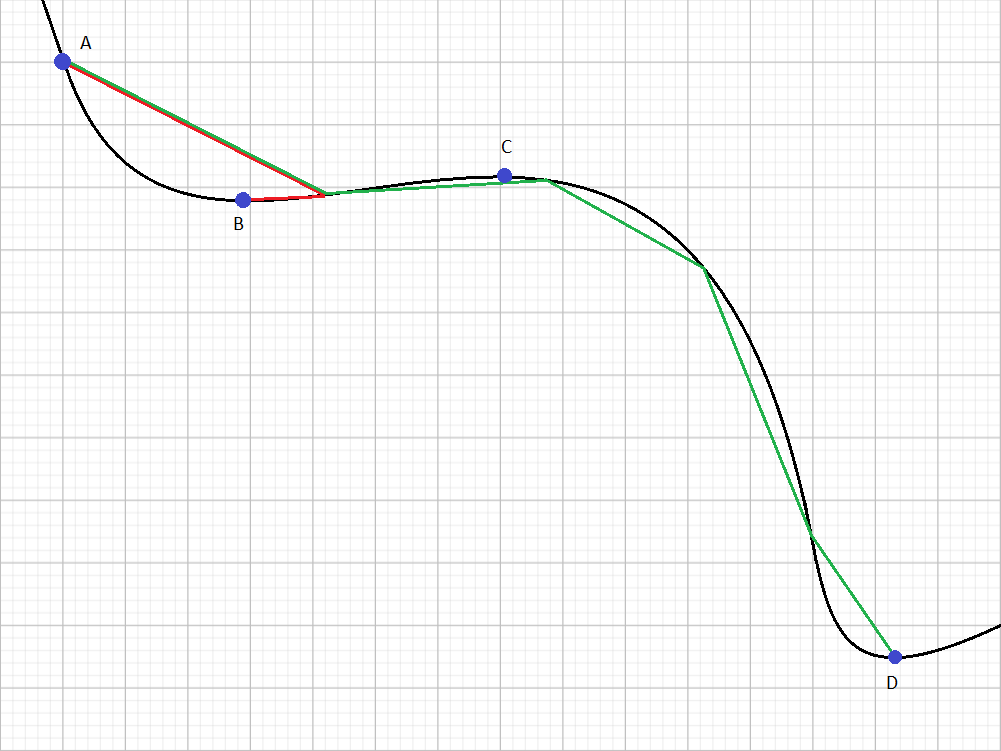
\includegraphics[width=\textwidth]{../img/gd_adam.png}
\caption{Ukážka rozdielu medzi algoritmami \textit{Gradient Descent} (červenou) a \textit{Adam} (zelenou). Čiernou farbou je znázornený graf hodnôt nejakej stratovej funkcie, A je bod, na ktorom obe algoritmy začínajú, B je lokálne minimum, C lokálne maximum a D globálne minimum. \textit{Adam} používa aj gradienty z minulých iterácií a tak je v tomto prípade schopný preskočiť lokálne maximum a pokračovať ďalej.}
\label{adam}
\end{figure}

Jedným z problémov neurónových sietí je to, že dosiahnuť ani len lokálne minimum nemusí byť požadujúce.
Ideálne požadujeme, aby sieť správne generalizovala, a teda aby jej výstup bol správny aj pre dáta, na ktorých sa neučila.
Aj keď trénovacia vzorka reprezentatuje realitu, môže sa stať, že sieť bude mať nízku hodnotu trénovacej chyby (stratovej funkcie), ale relatívne vysokú hodnotu testovacej chyby (príklad možno vidieť na obrázku \ref{overf}). Testovacia chyba sa vypočítava ako hodnota používanej stratovej funkcie na dátach, ktoré neboli obsiahnuté v trénovacej vzorke.
Tomuto fenoménu sa hovorí pretrénovanie (\textit{overfitting}) \citep{overfit}.
\noindent
\begin{figure} [h!]
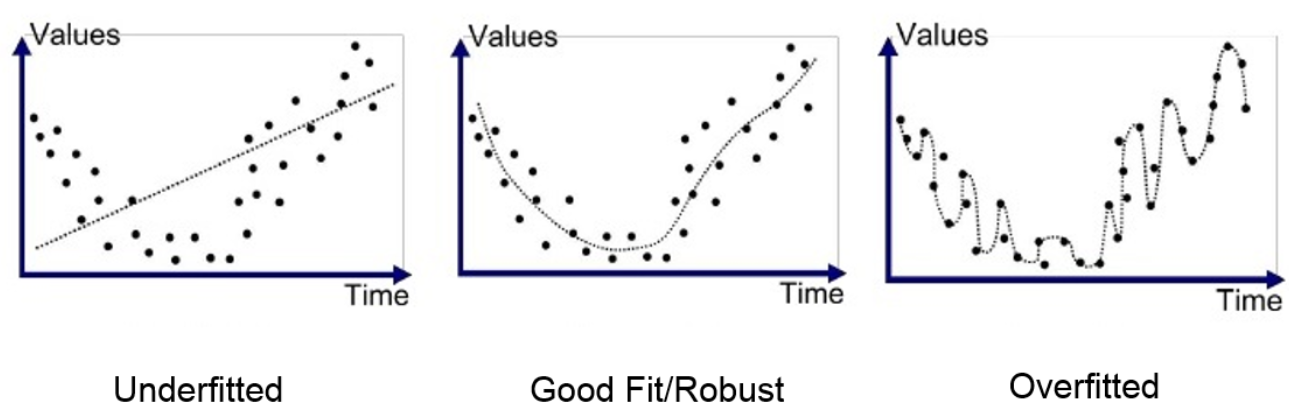
\includegraphics[width=\textwidth]{../img/overfit.png} 
\caption{Ukážka troch stavov, v ktorých sa môže sieť nachádzať: môže byť podtrénovaná (underfitted), správne natrénovaná (good fit) a pretrénovaná (overfitted) \citep{gitgud}.} 
\label{overf}
\end{figure}

Jedným zo spôsobov bojovania proti pretrénovaniu siete je použitie nejakej regularizačnej techniky. 
Regularizácia pomáha kontrolovať pretrénovanie siete \citep{overfit}.
Jednou z takýchto techník je napríklad technika zvaná \textit{dropout}.
\textit{Dropout} dostane spojenia od všetkých neurónov a náhodne zvolí, ktoré neuróny nedostanú svoje spojenie ďalej (ktorým neurónom nastaví váhy spojení na 0). Pre každú trénovaciu podmnožinu dát (\textit{batch}) to volí náhodne, takže na konci je veľmi veľká pravdepodobnosť, že každý neurón sa dostane ďalej a bude môcť byť jeho prísun evaluovaný a váha jeho spojenia pozmenená.